\section{\gls{fdtd} simulation} \label{sec:fdtd_simulation}
The aim of this section is to make a simulation of the zero order gradient speaker, first order gradient speaker and the solution proposed in \autoref{sec:opt_result} using \gls{fdtd}. All simulation across all three different methods of using speakers at low frequency will be compared in both free field and inside a room. The result will be discussed with respect to directionality and efficiency. 

\subsection{\gls{fdtd} step size}
This section will determine the the step size for both grid size and the time step size. Because the time step size is depending on the grid step size, the grid step size will be determined first. Recalling \autoref{fdtd_delta_stepsize} states, that all three dimention will have the same step size in this project. The calculation is as follows in\autoref{fdtd_distance_stepsize}.

\begin{subequations}\label{fdtd_distance_stepsize}
\begin{alignat}{2}
\delta d &= \delta x = \delta y = \delta z \leq \frac{1}{10} \frac{c}{f_{max}} \label{fdtd_distance_stepsize_1}\\
\delta d &= \frac{1}{10} \frac{\SI{343}{\meter\per\second}}{\SI{300}{\hertz}} \label{fdtd_distance_stepsize_2}\\
\delta d &= \SI{0.11}{\meter} \label{fdtd_distance_stepsize_3}
\end{alignat}
\end{subequations}

    \startexplain
    		\explain{$\ delta d$ is the maximum grid cell size }{\si{\meter}}
        \explain{$c$ is the speed of sound at a temperature of \SI{20}{\degree\celsius}}{\si{\meter\per\second}}
        \explain{$f_{max}$ is the maximum frequency in the simulation}{\si{\hertz}}
    \stopexplain

Since the maximum grid cell size is \SI{11}{\centi\meter}, the grid cell size is in this project will be less or equal to \SI{10}{\centi\meter}, to be sure that a simulation does not suffer from a limiting grid cell size. \\

From the optimization \autoref{sec:opt_result} it is determined that the optimal distance between the side speaker is \SI{40}{\centi\meter} and to the front speaker it is \SI{40}{\centi\meter}. When arranging the sources in a triangular shape, the greatest common divisor for putting them into a grid is \SI{20}{\centi\meter}. However this is bigger then than the formerly stated \SI{11}{\centi\meter}, which makes it unsuitable for simulation. Instead, it is decided to set the grid step size at \SI{5}{\centi\meter} in all simulations, to ensure flexibility during development. Next the time step has to be determined. The condition for the time step is stated in \autoref{fdtd_time_stepsize_boundary} and dictates the following \autoref{fdtd_time_stepsize_con_one}.
    
 
\begin{subequations}\label{fdtd_time_stepsize_con_one}
\begin{alignat}{2}
\delta t &\leq \sqrt{\frac{2}{3}}  \left( \frac{1}{\sqrt{\frac{1}{(\delta x)^2}+\frac{1}{(\delta x)^2}+\frac{1}{(\delta x)^2} }\cdot c} \right)\\
\delta t &\leq \sqrt{\frac{2}{3}}  \left( \frac{1}{\sqrt{\frac{1}{(\SI{0.05}{\meter})^2}+\frac{1}{(\SI{0.05}{\meter})^2}+\frac{1}{(\SI{0.05}{\meter})^2} }\cdot \SI{343}{\meter\per\second}} \right)\\
\delta t &\leq \SI{687}{\micro\second} 
\end{alignat}
\end{subequations}
    
A time step of \SI{687}{\micro\second}  corresponds to a sampling frequency of \SI{14552}{\hertz}. This sample frequency should make a stable simulation. It have been chosen to make a safety margin, and according to \autoref{fdtd_time_stepsize_con_one} lower sample frequency will make the simulation unstable, and therefore the sample frequency is only allowed to be higher. The sample frequency will be rounded up to \SI{14560}{\hertz}.
 
 

\subsection{\gls{fdtd} source}
The acoustic centers of the speakers will be represented as transparent sources, since a speaker cabinet \gls{fdtd} model will not be incorporated in this project. The source has a stability condition which has to be fulfilled and this includes the number of dimensions. In \autoref{sec:fdtd} the \gls{fdtd} is prepared to a three dimensions simulation, and all simulation will be done i three dimension.  The stability condition is stated in \autoref{fdtd_transparent_source_impulse_stability} and the stability achieved as shown in \autoref{fdtd_transparent_source_impulse_stability_calculation}.



\begin{subequations}\label{fdtd_transparent_source_impulse_stability_calculation}
\begin{alignat}{2}
\frac{c \delta t}{\delta d} &\leq \frac{1}{\sqrt{N}}\\
\frac{343 \cdot \SI{687}{\micro\second}}{\SI{5}{\centi\meter}} &\leq \frac{1}{\sqrt{3}}\\
0.471 &\leq 0.577
\end{alignat}
\end{subequations}

    \startexplain
    		\explain{$N$ is the number of dimension}{1}
    \stopexplain


As shown in \autoref{fdtd_transparent_source_impulse_stability_calculation} the transparent sound source is stable with the calculated time and grid size.

% The impulse response from the used \gls{dut} will be used as the impulse response in all simulation. All impulse response measurement in this project have a sample frequency of \SI{44.1}{\kilo\hertz} but because the simulation does not have to have higher sample frequency than \SI{7399}{\hertz}, the sample frequency of the measurement will be down sampled with a factor of 6. The choose of a factor of 6 is justified by that this is the highest scalar factor the measurement sampling frequency can be down sampled  and still satisfy the minimum sampling frequency and also keeping the required process power down. This result in a sampling frequency for the simulation of \SI{7.35}{\kilo\hertz}



\subsection{\gls{fdtd} implementation}
The aim of this section is to convert the grid to matrices. Since the grid is in three dimensions, where the time is a fourth dimension, the whole matrix system for pressure and all particle velocity matrices will built on four dimensional matrices. The following \autoref{fig:fdtd_cartesian_grid_matrice} shows a simple grid in a corner with entry notation of $h$ as the hight of the room, $w$ as the width of the room and $l$ as the length of the room.


\begin{figure}[H]
	\centering
\begin{picture}(0,0)%
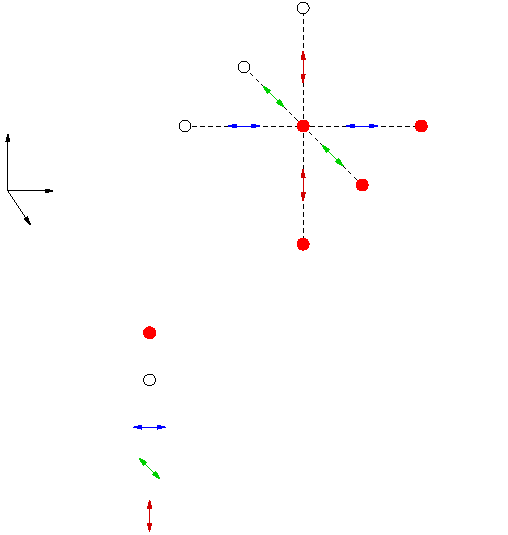
\includegraphics{fdtd_grid_matrices.pdf}%
\end{picture}%
\setlength{\unitlength}{4144sp}%
%
\begingroup\makeatletter\ifx\SetFigFont\undefined%
\gdef\SetFigFont#1#2#3#4#5{%
  \reset@font\fontsize{#1}{#2pt}%
  \fontfamily{#3}\fontseries{#4}\fontshape{#5}%
  \selectfont}%
\fi\endgroup%
\begin{picture}(3869,4070)(3541,-1873)
\put(5941,1334){\color[rgb]{0,0,1}$v_x(2,1,1)$}%
\put(4186,434){\color[rgb]{0,0,0}$(l,w,h)$}%
\put(5041,1019){\color[rgb]{0,0,1}$v_x(1,1,1)$}%
\put(6211,974){\color[rgb]{0,.82,0}$v_y(1,2,1)$}%
\put(5941,1604){\color[rgb]{.82,0,0}$v_z(1,1,1)$}%
\put(5041,749){\color[rgb]{.82,0,0}$v_z(1,1,2)$}%
\put(4771,1379){\color[rgb]{0,.82,0}$v_y(1,1,1)$}%
\put(5491, 74){\color[rgb]{1,0,0}$p(1,1,2)$}%
\put(6931,1199){\color[rgb]{1,0,0}$p(2,1,1)$}%
\put(6391,569){\color[rgb]{1,0,0}$p(1,2,1)$}%
\put(4996,-376){Pressure point}%
\put(4996,-736){Unknown pressure point}%
\put(3556,1244){$z$}%
\put(4996,-1096){Particle velocity x-direction}%
\put(4996,-1456){Particle velocity y-direction}%
\put(4006,704){$x$}%
\put(3826,344){$y$}%
\put(4996,-1771){Particle velocity z-direction}%
\end{picture}%
	\caption{The figure visualized a boundary plan through particle velocity plan $x$ in 1 dimension}
		\label{fig:fdtd_cartesian_grid_matrice}
\end{figure}

All simulation is implemented in MATLAB. The $x$ direction is implemented as matrix row direction and $y$ direction is implemented as matrix column direction. The height $h$ is implemented as the third dimension and the time is implemented as the fourth dimension. The particle velocity will be calculated as the first step and the pressure will be calculated as the second step. The time dimension is only as small as 2 pages, because it is only necessary to save at $[l-1]$ and at $[l]$. A page is one dimension in a matrix system, where the number before ´´page"  describes the time in this context and not a two dimension page. There can be many dimensions for pages, where the implementation of the \gls{fdtd} has two page dimensions.  All time steps further away than $[l-1]$ are not used in the calculation and will be deleted for keeping the storage requirements as low as possible. 

\subsection{\gls{fdtd} boundary}
The particle velocity at the boundary in all direction has to be calculated as in \autoref{fdtd_boundary_result} and this is done as a step between the particle velocity matrices and the pressure matrices. This means, that for the particle velocity in $x$ direction the first and last matrix row are calculated by the boundary formula and in $y$ direction the first column and the last matrix column is calculated by the boundary formula. 


\subsection{\gls{fdtd} plot}
The aim of the section is to explain how the phase, gain and distance, resulting from \autoref{ch:optimization}, are implemented in the \gls{fdtd} simulation, and how the result of the simulation is compared with the polar plot from \autoref{ch:optimization}. \\

To be able to simulate the result from \autoref{ch:optimization}, three pressure points is used as the acoustical center. The pressure points are implemented as transparent point sources, where all the point sources is fed with a sinusoid of a single frequency where the phase and gain is adjusted to the specified frequency. The front speakers will always be feeded with a gain of one, which correspond to a pressure of $\pm \SI{1}{\pascal}$ and zero phase. Therefore it is only the back speaker, which will be adjusted in phase and gain. The number of simulation run steps is the smallest room size divided by the grid size, such that the waves do not reflect from the wall. \\

A wave will expand in a circular form and since the simulation stops just before the it hits the first wall, the simulation result will be a circular shape. Some of the area is not simulated and is therefore without a valid pressure. Because of this, the simulation is made so large that the polar plot with a radius of \SI{10}{\meter} can still be calculated, where the used simulation data is only a squared area inside the circular shape and the rest data is discarded.\\

The polar plot from the analytical model is based on the \gls{rms} pressure, therefore the \gls{rms} pressure of the \gls{fdtd} has to be calculated. The \gls{rms} of the \gls{fdtd} simulation is calculated as following in \autoref{fdtd_rms_pressure}.

\begin{equation}\label{fdtd_rms_pressure}
P_{rms}(i,j,k)=\sqrt{\frac{\left(p_{(i,j,k)}^{[l= \delta t]} \right))^2 + \left(p_{(i,j,k)}^{[l= 2\delta t]}\right)^2 +...+\left(p_{(i,j,k)}^{[l= n\delta t]}\right)^2}{n}}
\end{equation}


\subsection{The three speaker model} \label{the_simulation_result}
In this section, the three speaker array simulation result will be presented and compared to the analytical model. The following figures show the results from \SI{60}{\hertz} to \SI{300}{\hertz} with a frequency step of \SI{50}{\hertz} from \SI{100}{\hertz}. Beneath \SI{100}{\hertz} the step is \SI{40}{\hertz}. All results have been achieved according to the description in this chapter. All polar plots are normalized, so that they only show the attenuation all around the circumference. The exact pressure from the analytical model and the \gls{fdtd} simulation will be stated in the caption of every figure. 


Until now the analytical model have been based on relative pressure. This have been done because the radius of the acoustical center sphere have been unknown. At this point it is now possible to estimate the acoustical sphere radius for this problem by solving 'a' in \autoref{eq:aug_omni} with knowing the frequency, the pressure on the main axis at a distance of \SI{10}{\meter} by doing a \gls{fdtd} simulating. It have been chosen that the acoustical center sphere shall be solved from \SI{60}{\hertz}. The particle velocity is calculated from the impedance relation, which state

\begin{equation}
Z_{air}=\frac{p_a}{v}
\end{equation}  

    \startexplain
    		\explain{$Z_{air}$ is the air impedance}{1}
    		\explain{$p_a$ is the sound pressure at a distance of \SI{10}{\meter} of the analytical model}{\si{\pascal}}
    		\explain{$v$ is the velocity}{1}
    \stopexplain

The sphere radius 'a' is solved to be \SI{7.6}{\milli\meter}. The following ploar plot will both show the absolute and the relative pressure for both the analytical model and the \gls{fdtd} simulation




\begin{figure}[H]
\centering
\begin{subfigure}[htbp]{0.55\textwidth}
		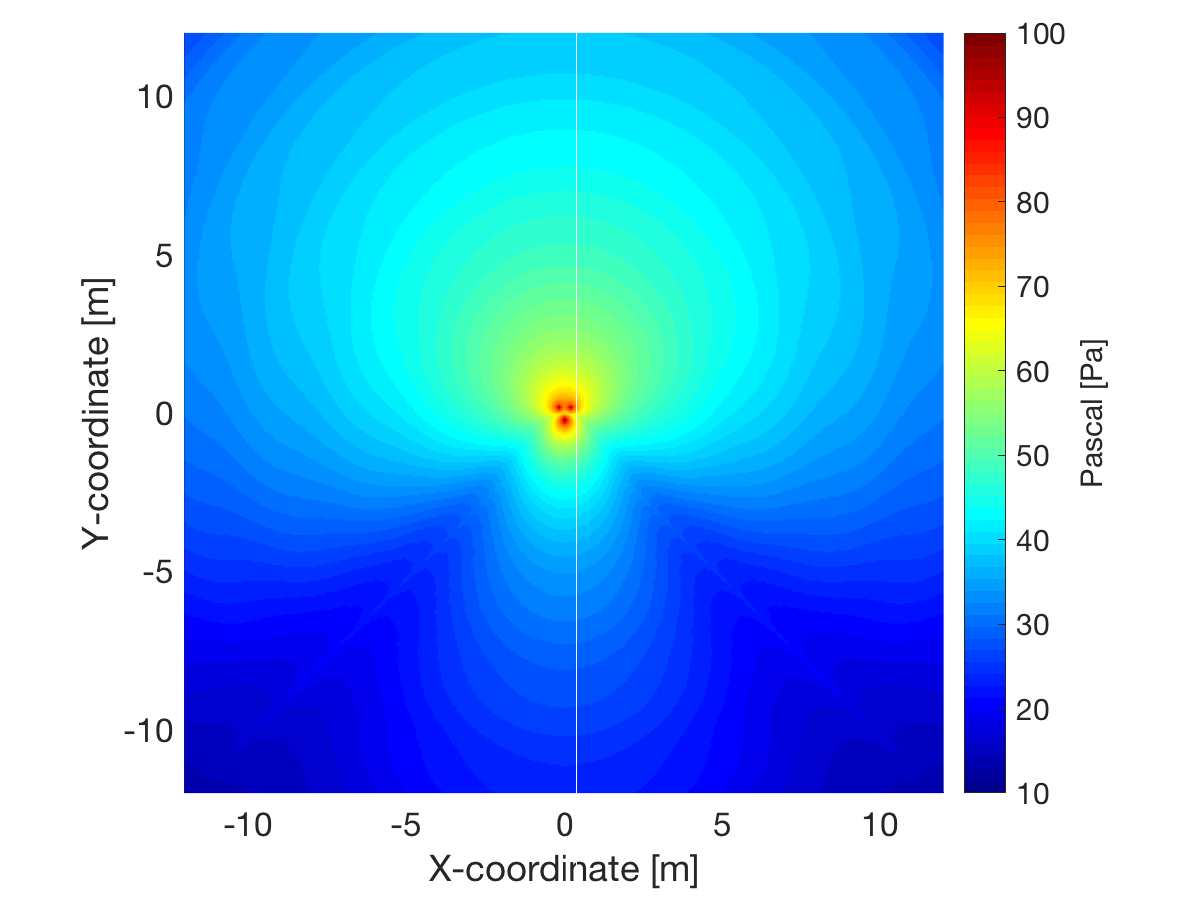
\includegraphics[width=\textwidth]{60_hz_fdtd_plot.eps}
		\caption{The figure shows the \gls{fdtd} simulation of \SI{60}{\hertz}}
		\label{fig:fdtd_60_Hz}
\end{subfigure}
\begin{subfigure}[htbp]{0.35\textwidth}
		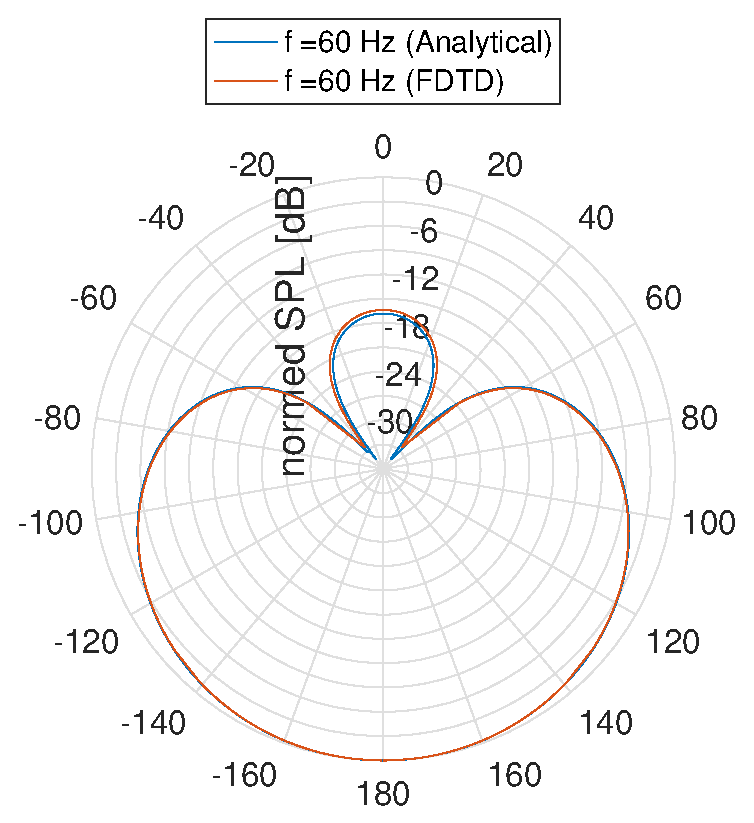
\includegraphics[width=\textwidth]{60_hz_polar_plot.eps}
		\caption{The figure shows the analytical- and \gls{fdtd} polar plot at \SI{60}{\hertz} with a radius of \SI{10}{\meter}}
		\label{fig:polar_60_Hz}
\end{subfigure} 
\caption{The figure compares the analytical model and the \gls{fdtd} model of speaker array at \SI{60}{\hertz}}
\end{figure}


\begin{figure}[H]
\centering
\begin{subfigure}[htbp]{0.55\textwidth}
		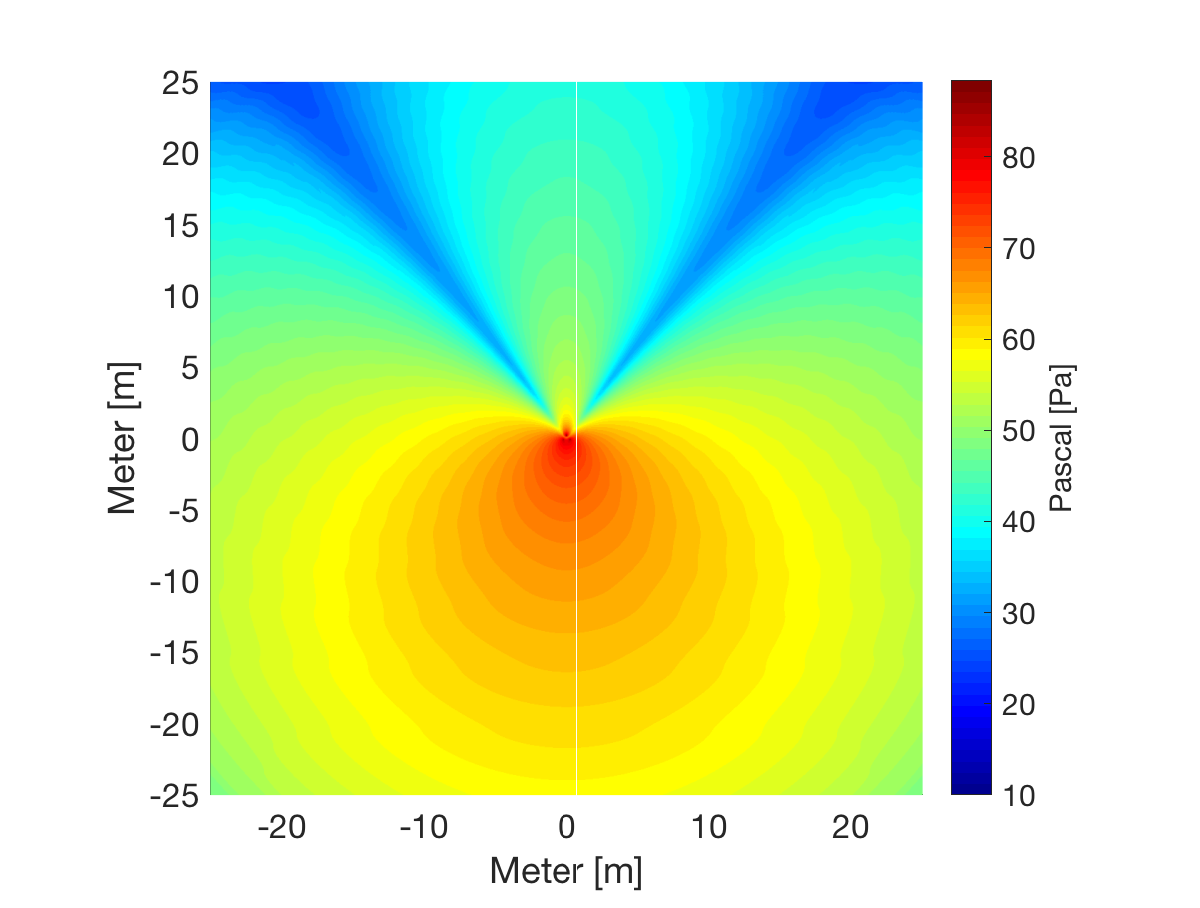
\includegraphics[width=\textwidth]{100_hz_fdtd_plot.eps}
		\caption{The figure shows the \gls{fdtd} simulation of \SI{70}{\hertz}}
		\label{fig:fdtd_100_Hz}
\end{subfigure}
\begin{subfigure}[htbp]{0.35\textwidth}
		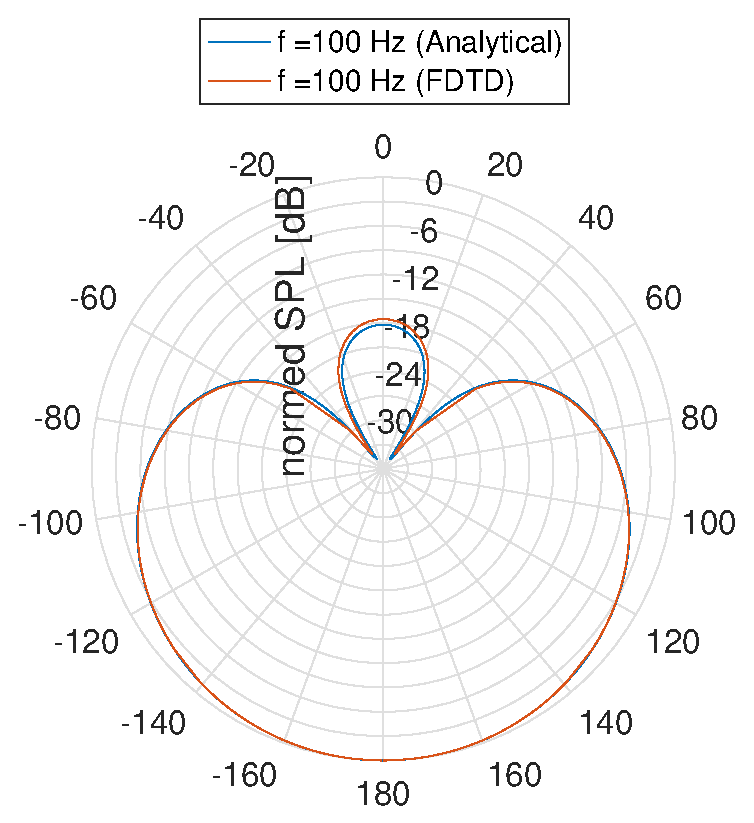
\includegraphics[width=\textwidth]{100_hz_polar_plot.eps}
		\caption{The figure shows the analytical- and \gls{fdtd} polar plot at \SI{70}{\hertz} with a radius of \SI{10}{\meter}}
		\label{fig:polar_100_Hz}
\end{subfigure} 
\caption{The figure compares the analytical model and the \gls{fdtd} model of the speaker array at \SI{100}{\hertz}}
\end{figure}


\begin{figure}[H]
\centering
\begin{subfigure}[htbp]{0.55\textwidth}
		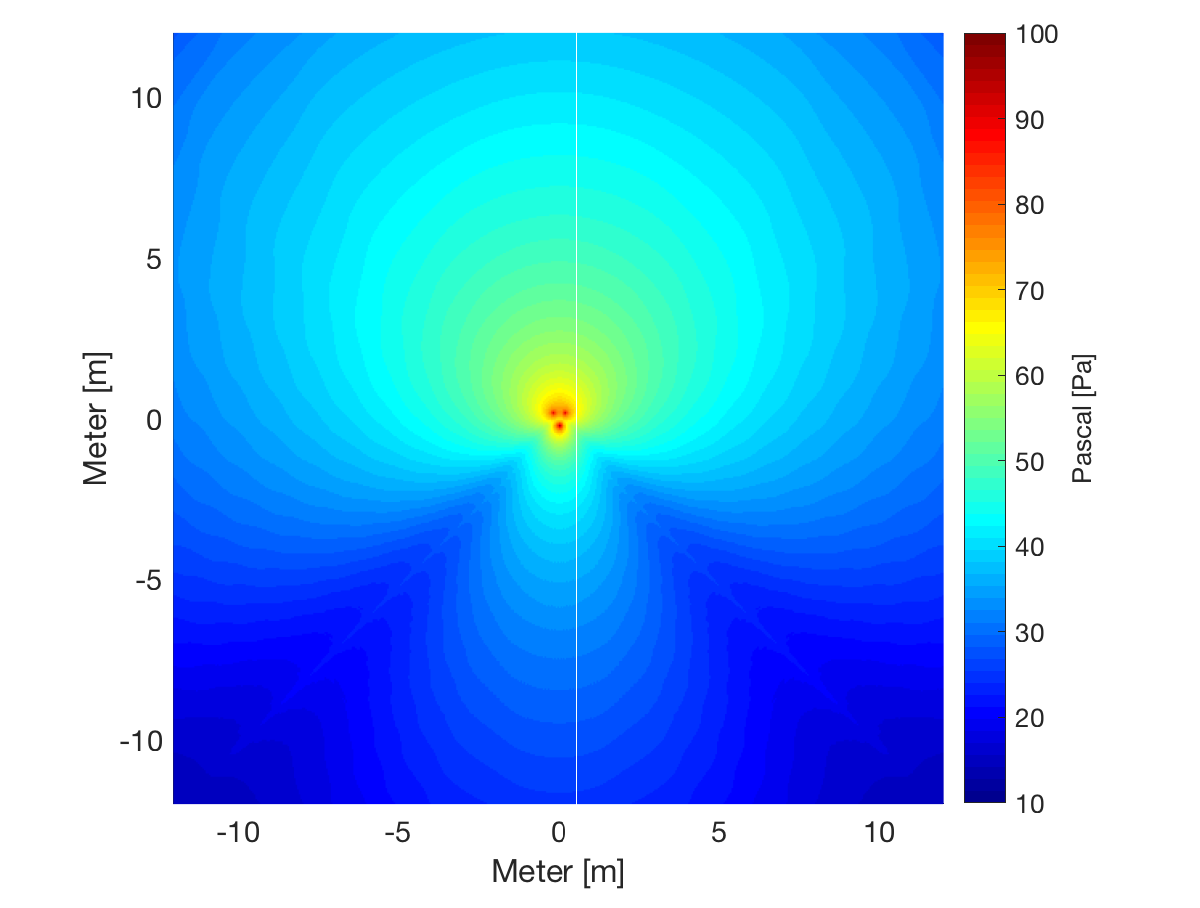
\includegraphics[width=\textwidth]{150_hz_fdtd_plot.eps}
		\caption{The figure shows the \gls{fdtd} simulation of \SI{80}{\hertz}}
		\label{fig:fdtd_150_Hz}
\end{subfigure}
\begin{subfigure}[htbp]{0.35\textwidth}
		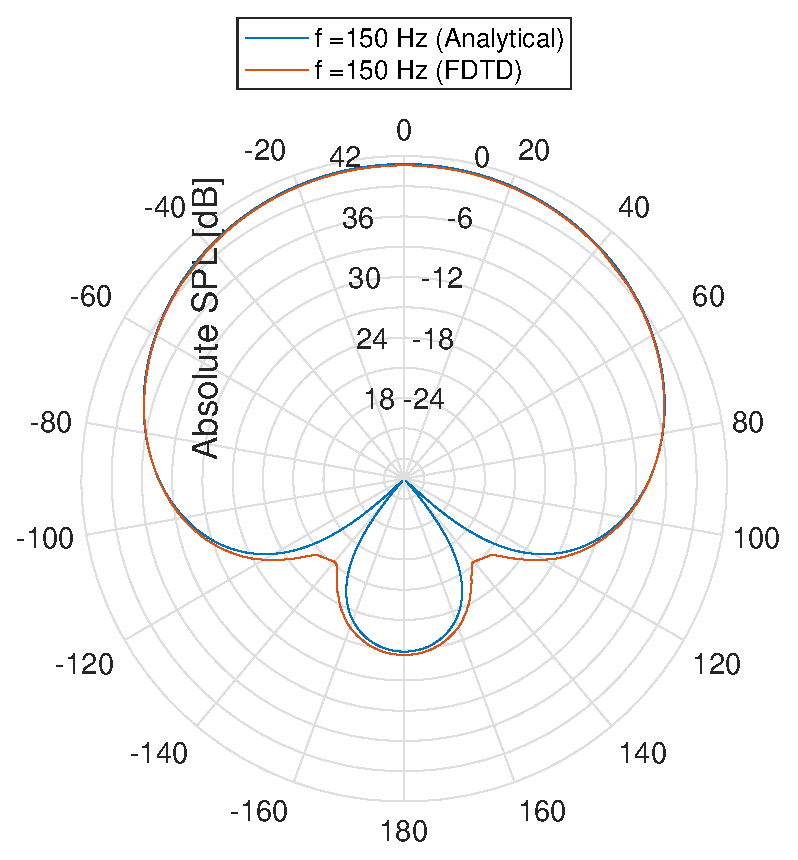
\includegraphics[width=\textwidth]{150_hz_polar_plot.eps}
		\caption{The figure shows the analytical- and \gls{fdtd} polar plot at \SI{80}{\hertz} with a radius of \SI{10}{\meter}}
		\label{fig:polar_150_Hz}
\end{subfigure} 
\caption{The figure compares the analytical model and the \gls{fdtd} model of the speaker array at \SI{150}{\hertz}}
\end{figure}


\begin{figure}[H]
\centering
\begin{subfigure}[htbp]{0.55\textwidth}
		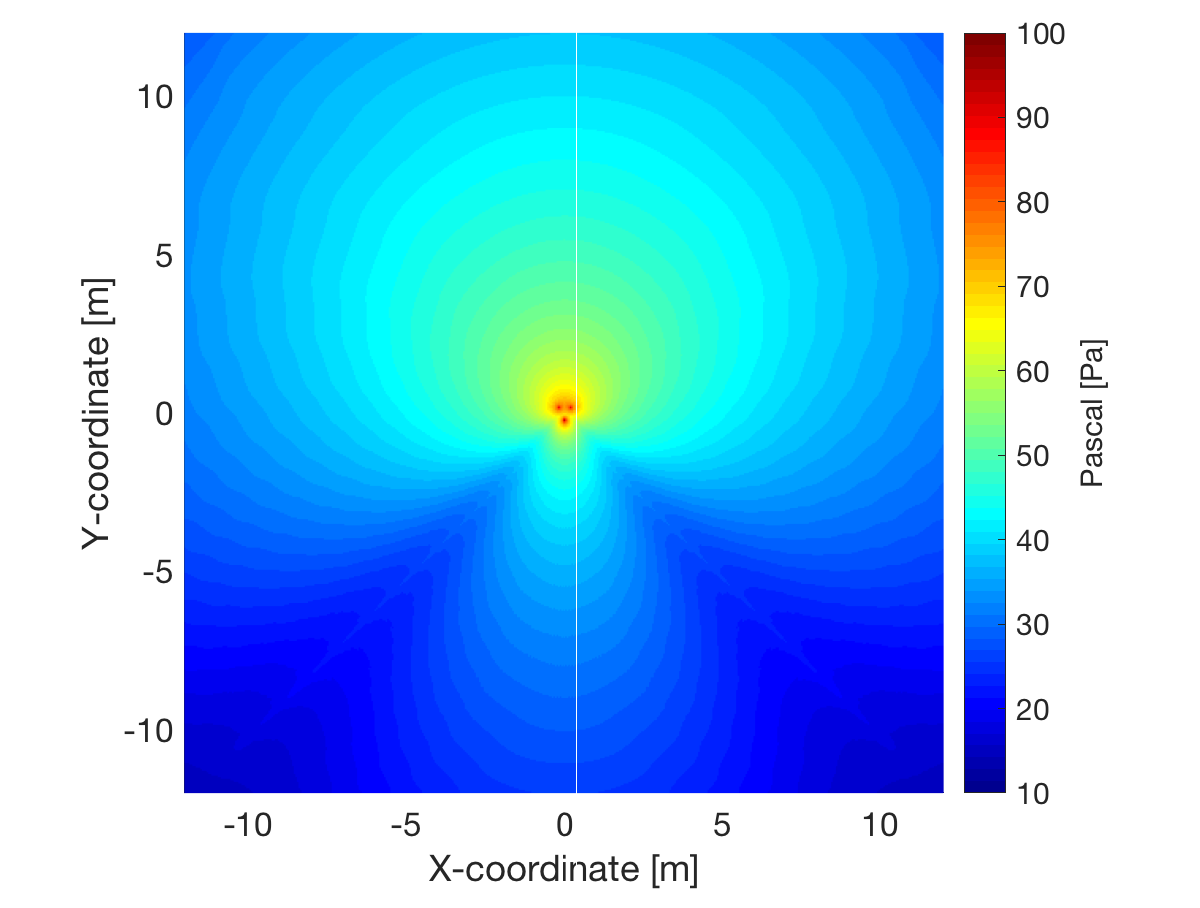
\includegraphics[width=\textwidth]{200_hz_fdtd_plot.eps}
		\caption{The figure shows the \gls{fdtd} simulation of \SI{90}{\hertz}}
		\label{fig:fdtd_200_Hz}
\end{subfigure}
\begin{subfigure}[htbp]{0.35\textwidth}
		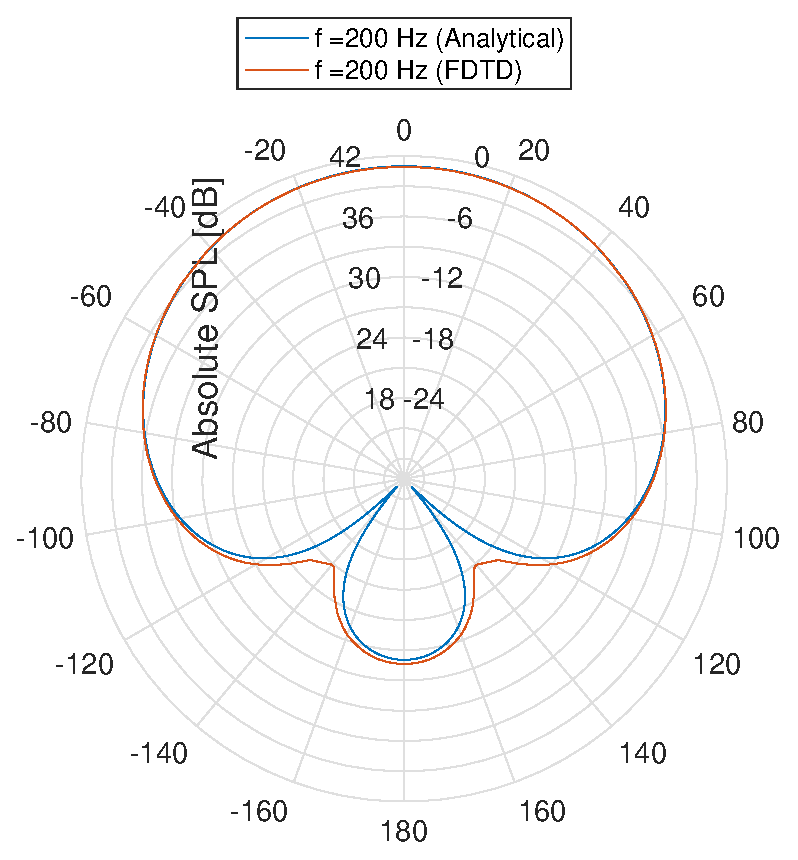
\includegraphics[width=\textwidth]{200_hz_polar_plot.eps}
		\caption{The figure shows the analytical- and \gls{fdtd} polar plot at \SI{90}{\hertz} with a radius of \SI{10}{\meter}}
		\label{fig:polar_200_Hz}
\end{subfigure} 
\caption{The figure compares the analytical model and the \gls{fdtd} model of the speaker array model at \SI{200}{\hertz}}
\end{figure}


\begin{figure}[H]
\centering
\begin{subfigure}[htbp]{0.55\textwidth}
		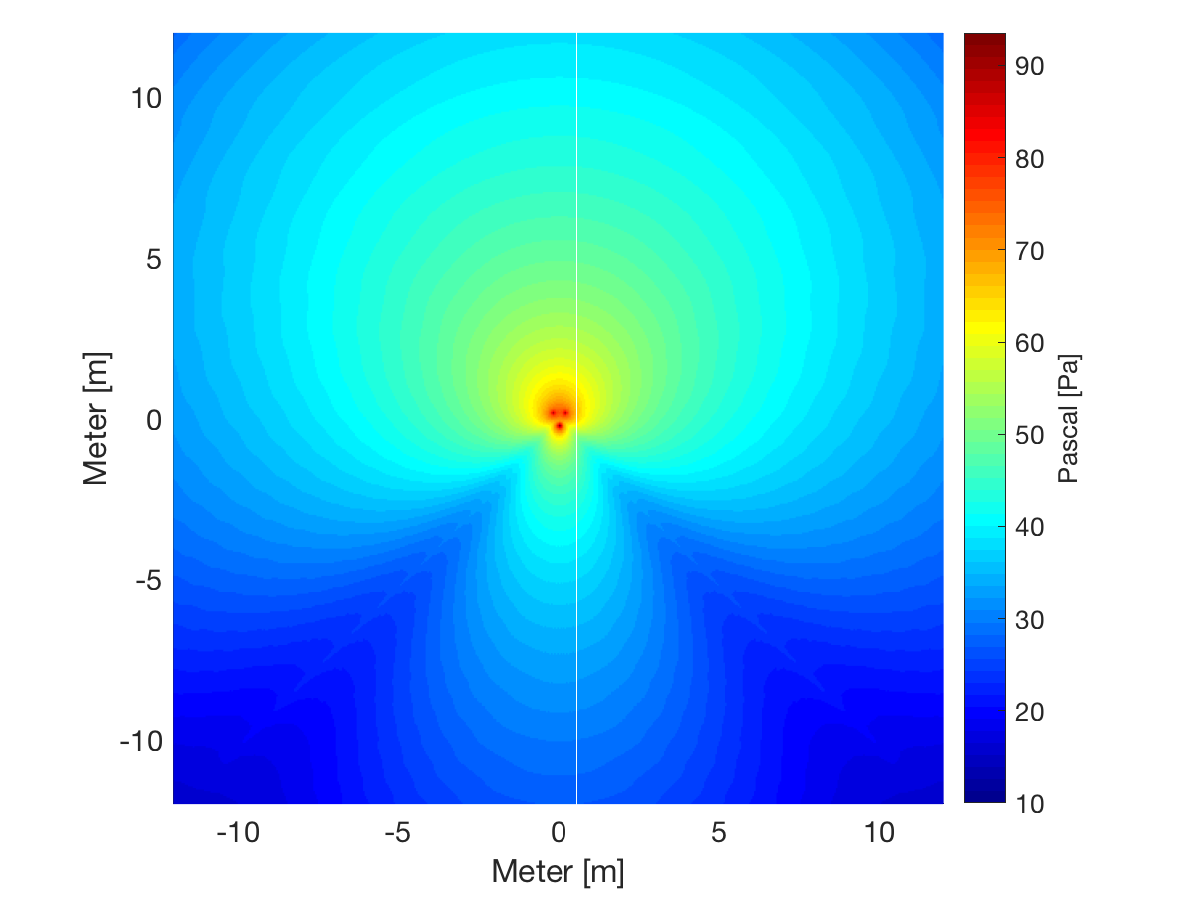
\includegraphics[width=\textwidth]{250_hz_fdtd_plot.eps}
		\caption{The figure shows the \gls{fdtd} simulation of \SI{100}{\hertz}}
		\label{fig:fdtd_250_Hz}
\end{subfigure}
\begin{subfigure}[htbp]{0.35\textwidth}
		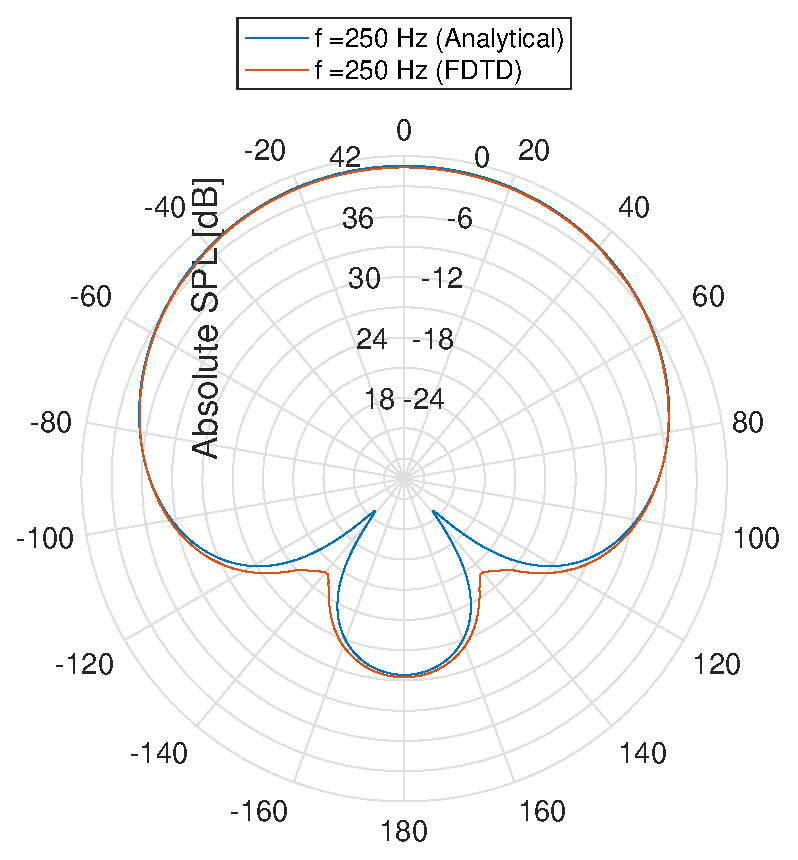
\includegraphics[width=\textwidth]{250_hz_polar_plot.eps}
		\caption{The figure shows the analytical- and \gls{fdtd} polar plot at \SI{100}{\hertz} with a radius of \SI{10}{\meter}}
		\label{fig:polar_250_Hz}
\end{subfigure} 
\caption{The figure compares the analytical model and the \gls{fdtd} model of the speaker array at \SI{250}{\hertz}}
\end{figure}


\begin{figure}[H]
\centering
\begin{subfigure}[htbp]{0.55\textwidth}
		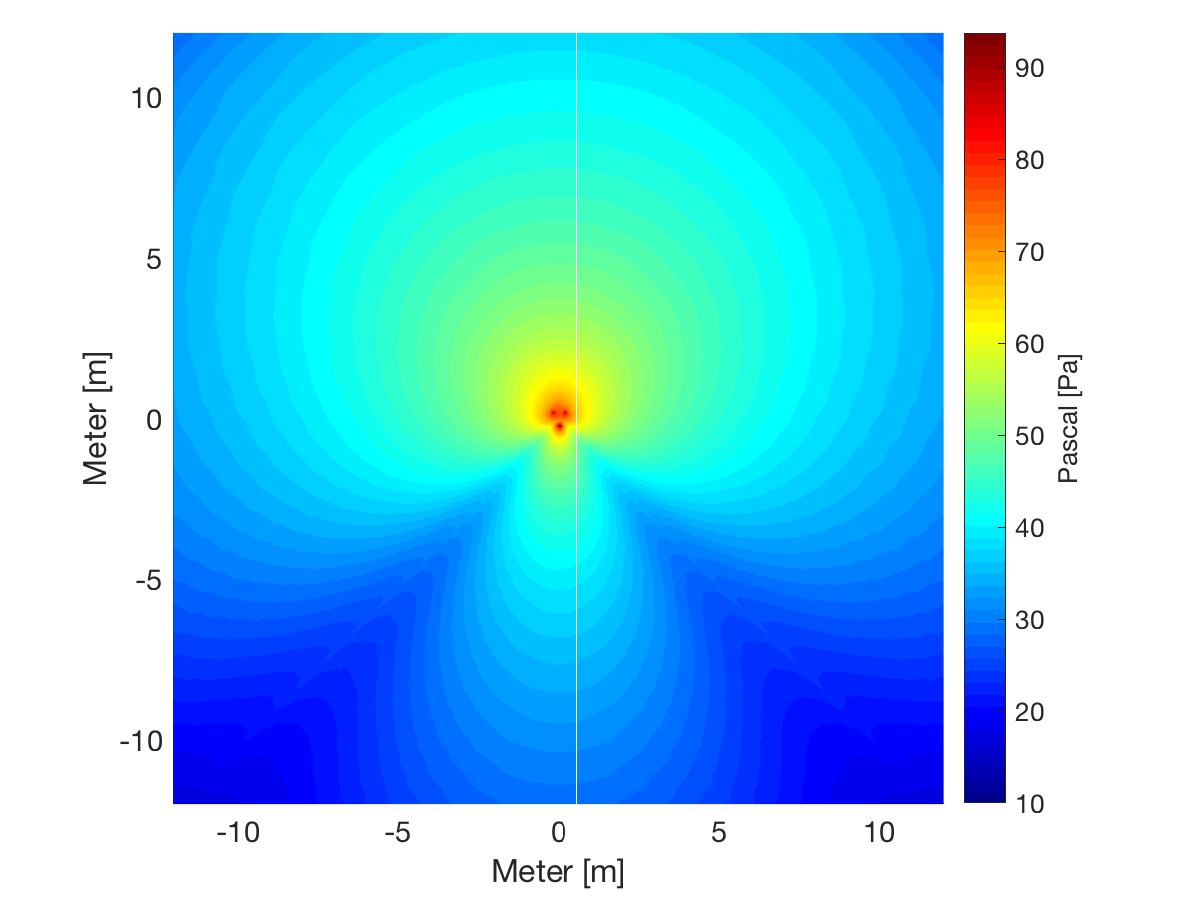
\includegraphics[width=\textwidth]{300_hz_fdtd_plot.eps}
		\caption{The figure shows the \gls{fdtd} simulation of \SI{100}{\hertz}}
		\label{fig:fdtd_300_Hz}
\end{subfigure}
\begin{subfigure}[htbp]{0.35\textwidth}
		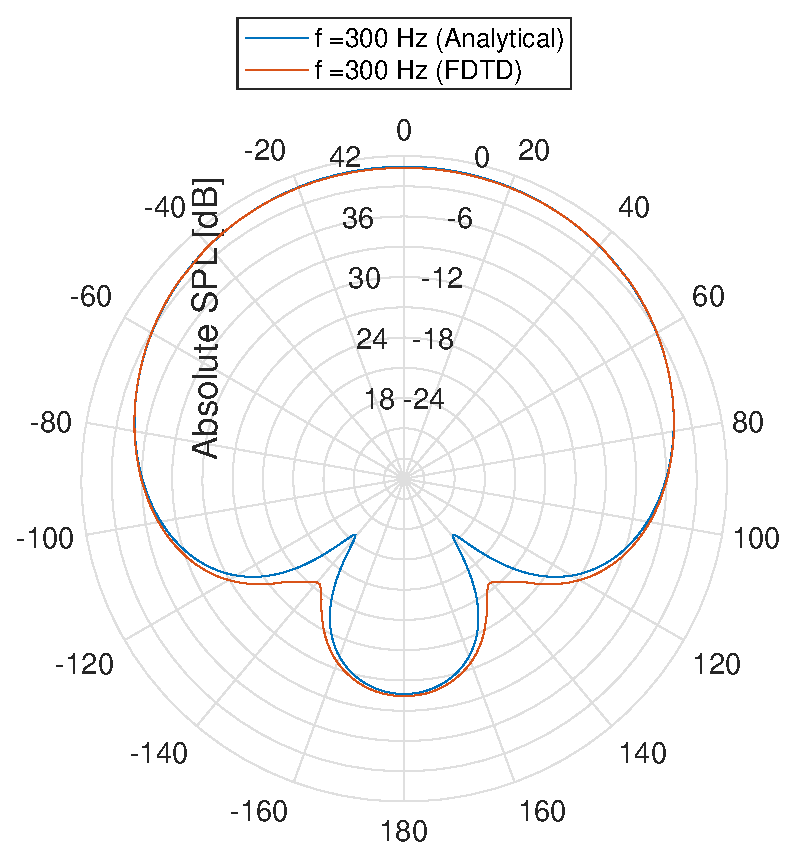
\includegraphics[width=\textwidth]{300_hz_polar_plot.eps}
		\caption{The figure shows the analytical- and \gls{fdtd} polar plot at \SI{100}{\hertz} with a radius of \SI{10}{\meter}}
		\label{fig:polar_300_Hz}
\end{subfigure} 
\caption{The figure compares the analytical model and the \gls{fdtd} model of the speaker array at \SI{300}{\hertz}}
\end{figure}

\section{Conclusion}
It can be concluded that the simulation agrees with the analytical model. The side depth of the simulation is not as deep as on the analytical model, but this due the the simulation time. The longer the simulation runs, the more similar the shape for the simulated polar plot and the polar plot of the analytical model gets. More simulation can be founded in the \autoref{ap:fdtd_in_between} where simulation figure of other than the polar plot resolution is presented.


